% RL2025 Lecture 2: Deep Learning Essentials
\documentclass[aspectratio=169,10pt]{beamer}

% Essential packages
\usepackage[utf8]{inputenc}
\usepackage[T1]{fontenc}
\usepackage{amsmath,amssymb,amsthm}
\usepackage{graphicx}
\usepackage{listings}
\usepackage{xcolor}
\usepackage{tikz}
\usepackage{algorithm}
\usepackage{algorithmic}
\usepackage{hyperref}

% Use mimic.sty to prevent overfull boxes
\usepackage{mimic}

% Theme configuration
\usetheme{Madrid}
\usecolortheme{seahorse}
\setbeamertemplate{navigation symbols}{}
\setbeamertemplate{footline}[frame number]

% Code listing settings
\lstset{
    language=Python,
    basicstyle=\ttfamily\scriptsize,
    keywordstyle=\color{blue}\bfseries,
    stringstyle=\color{red},
    commentstyle=\color{green!60!black},
    showstringspaces=false,
    breaklines=true,
    breakatwhitespace=true,
    frame=single,
    numbers=left,
    numberstyle=\tiny\color{gray},
    xleftmargin=1em,
    framexleftmargin=1em
}

% Title page information
\title{Reinforcement Learning}
\subtitle{Lecture 2: Deep Learning Essentials}
\author{Taehoon Kim}
\institute{Sogang University MIMIC Lab \\ \url{https://mimic-lab.com}}
\date{Fall Semester 2025}
\begin{document}

% ============================================
% FRONT MATTER (Slides 1-3)
% ============================================

% Slide 1: Title page
\frame{\titlepage}

% Slide 3: Learning Objectives
\begin{frame}{Learning Objectives}
\begin{block}{By the end of this lecture, you will:}
\begin{itemize}
    \item Understand tensor operations and automatic differentiation
    \item Master PyTorch's nn.Module system
    \item Implement gradient checking for verification
    \item Build complete training pipelines with proper device handling
    \item Apply regularization and initialization techniques
    \item Complete 9 hands-on experiments
\end{itemize}
\end{block}

\begin{alertblock}{Prerequisites}
\begin{itemize}
    \item Python programming experience
    \item Basic linear algebra (matrix operations)
    \item Calculus (derivatives and chain rule)
\end{itemize}
\end{alertblock}
\end{frame}

% ============================================
% SECTION 1: Tensors and PyTorch (Slides 4-20)
% ============================================
\section{Tensors and PyTorch Fundamentals}

% Slide 4: Section introduction
\begin{frame}{Tensors and PyTorch Fundamentals}
\begin{center}
\Large{The Foundation of Deep Learning}
\end{center}

\begin{block}{Topics}
\begin{itemize}
    \item What are tensors?
    \item PyTorch tensor operations
    \item Device management
    \item Broadcasting and shape manipulation
\end{itemize}
\end{block}
\end{frame}

% Slide 5: What is a Tensor?
\begin{frame}{What is a Tensor?}
\textbf{Definition:} Multidimensional array with hardware acceleration support

\begin{itemize}
    \item \textbf{Scalar:} 0D tensor (single number)
    \item \textbf{Vector:} 1D tensor [n]
    \item \textbf{Matrix:} 2D tensor [m, n]
    \item \textbf{3D Tensor:} [batch, height, width]
    \item \textbf{4D Tensor:} [batch, channels, height, width]
\end{itemize}

\begin{block}{Key Properties}
\begin{itemize}
    \item Device placement (CPU, CUDA, MPS)
    \item Data type (float32, float64, int64, etc.)
    \item Gradient tracking (requires\_grad)
\end{itemize}
\end{block}
\end{frame}

% Slide 6: Creating Tensors
\begin{frame}[fragile]{Creating Tensors}
\begin{lstlisting}
import torch

# From data
x = torch.tensor([1, 2, 3])           # From list
y = torch.tensor([[1, 2], [3, 4]])    # 2D tensor

# Random tensors
z = torch.randn(3, 4)    # Normal distribution
u = torch.rand(2, 3)     # Uniform [0, 1)

# Special tensors
zeros = torch.zeros(3, 3)
ones = torch.ones(2, 4)
eye = torch.eye(3)       # Identity matrix

# With specific dtype and device
x = torch.tensor([1.0], dtype=torch.float64,
                 device='cuda' if torch.cuda.is_available() 
                 else 'cpu')
\end{lstlisting}
\end{frame}

% Slide 7: Tensor Operations
\begin{frame}[fragile]{Tensor Operations}
\begin{lstlisting}
# Basic arithmetic
a = torch.tensor([1., 2., 3.])
b = torch.tensor([4., 5., 6.])

c = a + b          # Element-wise addition
d = a * b          # Element-wise multiplication
e = a @ b          # Dot product (same as torch.dot)

# Matrix operations
A = torch.randn(3, 4)
B = torch.randn(4, 5)
C = A @ B          # Matrix multiplication [3, 5]

# In-place operations (use with caution!)
a.add_(1)          # Modifies a in-place
a.mul_(2)          # Dangerous with autograd!
\end{lstlisting}
\end{frame}

% Slide 8: Device Management
\begin{frame}[fragile]{Device Management}
\begin{lstlisting}
# Proper device selection (CUDA > MPS > CPU)
device = torch.device(
    'cuda' if torch.cuda.is_available() 
    else 'mps' if hasattr(torch.backends, 'mps') 
                  and torch.backends.mps.is_available()
    else 'cpu'
)

# Moving tensors between devices
x = torch.randn(3, 4)
x = x.to(device)           # Move to selected device
x = x.cpu()                # Back to CPU

# Creating directly on device
y = torch.randn(3, 4, device=device)

# Check device
print(x.device)            # cuda:0 or cpu
print(x.is_cuda)          # True/False
\end{lstlisting}
\end{frame}

% Slide 9: Broadcasting
\begin{frame}[fragile]{Broadcasting Rules}
PyTorch automatically expands tensors for element-wise operations:

\begin{lstlisting}
# Scalar broadcast
a = torch.randn(3, 4)
b = 2.0
c = a * b              # b broadcasts to [3, 4]

# Vector broadcast
a = torch.randn(3, 4)  # [3, 4]
b = torch.randn(4)     # [4] -> broadcasts to [3, 4]
c = a + b              # OK

# Matrix broadcast
a = torch.randn(3, 1, 4)  # [3, 1, 4]
b = torch.randn(1, 5, 4)  # [1, 5, 4]
c = a + b                  # [3, 5, 4]
\end{lstlisting}

\textbf{Rule:} Dimensions are compatible if they are equal or one is 1
\end{frame}

% Slide 10: Shape Manipulation
\begin{frame}[fragile]{Shape Manipulation}
\begin{lstlisting}
x = torch.randn(12)

# Reshape (creates new tensor if needed)
y = x.reshape(3, 4)      # [12] -> [3, 4]
y = x.reshape(2, 2, 3)   # [12] -> [2, 2, 3]

# View (shares memory, must be contiguous)
z = x.view(3, 4)         # [12] -> [3, 4]

# Add/remove dimensions
a = torch.randn(3, 4)
b = a.unsqueeze(0)       # [3, 4] -> [1, 3, 4]
c = b.squeeze(0)         # [1, 3, 4] -> [3, 4]

# Transpose and permute
d = a.T                  # Transpose (2D only)
e = a.transpose(0, 1)    # Swap specific dims
f = a.permute(1, 0)      # Reorder dimensions
\end{lstlisting}
\end{frame}

% Slide 11: Indexing and Slicing
\begin{frame}[fragile]{Indexing and Slicing}
\begin{lstlisting}
x = torch.randn(3, 4, 5)

# Basic indexing
a = x[0]               # First batch: [4, 5]
b = x[:, 0, :]         # First row: [3, 5]
c = x[..., -1]         # Last column: [3, 4]

# Advanced indexing
indices = torch.tensor([0, 2])
d = x[indices]         # Select batches 0 and 2

# Boolean masking
mask = x > 0
positive = x[mask]     # All positive values

# Gather and scatter
idx = torch.tensor([[0, 1], [2, 0]])
gathered = torch.gather(x[0], 0, idx)
\end{lstlisting}
\end{frame}

% Slide 12: Memory and Performance
\begin{frame}{Memory and Performance Tips}
\begin{itemize}
    \item \textbf{Contiguous memory:} Use \texttt{.contiguous()} after transpose
    \item \textbf{In-place operations:} Suffix with \_ but avoid with autograd
    \item \textbf{No gradient:} Use \texttt{torch.no\_grad()} for inference
    \item \textbf{Half precision:} Use \texttt{float16} or \texttt{bfloat16} for speed
    \item \textbf{Pin memory:} Use \texttt{pin\_memory=True} in DataLoader
\end{itemize}

\begin{block}{Common Pitfalls}
\begin{itemize}
    \item Forgetting to move model and data to same device
    \item In-place operations breaking gradient computation
    \item Memory leaks from retaining gradients
    \item Not using \texttt{torch.no\_grad()} during evaluation
\end{itemize}
\end{block}
\end{frame}

% Slide 13: Seeding for Reproducibility
\begin{frame}[fragile]{Reproducibility Setup}
\begin{lstlisting}
import os, random, numpy as np, torch

def setup_seed(seed=42):
    random.seed(seed)
    np.random.seed(seed)
    torch.manual_seed(seed)
    if torch.cuda.is_available():
        torch.cuda.manual_seed_all(seed)
        # For exact reproducibility (slower)
        torch.backends.cudnn.deterministic = True
        torch.backends.cudnn.benchmark = False

# Call at start of script
setup_seed(42)

# Also set environment variables
os.environ['PYTHONHASHSEED'] = str(42)
\end{lstlisting}
\end{frame}

% Slide 14: Tensor Attributes
\begin{frame}[fragile]{Tensor Attributes and Metadata}
\begin{lstlisting}
x = torch.randn(3, 4, 5, requires_grad=True)

# Shape information
print(x.shape)          # torch.Size([3, 4, 5])
print(x.size())         # torch.Size([3, 4, 5])
print(x.ndim)           # 3 (number of dimensions)
print(x.numel())        # 60 (total elements)

# Data type and device
print(x.dtype)          # torch.float32
print(x.device)         # cpu or cuda:0
print(x.layout)         # torch.strided

# Gradient information
print(x.requires_grad)  # True
print(x.grad)           # None (before backward)
print(x.is_leaf)        # True (user-created)
\end{lstlisting}
\end{frame}

% Slide 15: Type Casting
\begin{frame}[fragile]{Type Casting and Conversion}
\begin{lstlisting}
# Create tensor with specific type
x = torch.tensor([1, 2, 3], dtype=torch.float64)

# Type conversion
y = x.float()          # Convert to float32
z = x.long()           # Convert to int64
w = x.half()           # Convert to float16

# To/from NumPy (shares memory on CPU!)
np_array = x.numpy()          # Tensor -> NumPy
tensor = torch.from_numpy(np_array)  # NumPy -> Tensor

# To Python scalars
scalar_tensor = torch.tensor(3.14)
python_float = scalar_tensor.item()  # Extract value

# Detach from computation graph
x_detached = x.detach()       # No gradient tracking
\end{lstlisting}
\end{frame}

% Slide 16: Tensor Comparison
\begin{frame}[fragile]{Tensor Comparison Operations}
\begin{lstlisting}
a = torch.tensor([1, 2, 3])
b = torch.tensor([3, 2, 1])

# Element-wise comparison
print(a == b)          # [False, True, False]
print(a > b)           # [False, False, True]
print(a <= b)          # [True, True, False]

# Aggregated comparisons
print(torch.all(a == b))      # False
print(torch.any(a == b))      # True

# Close comparison (for floats)
c = torch.tensor([1.0, 2.0, 3.0])
d = torch.tensor([1.0001, 2.0, 3.0])
print(torch.allclose(c, d, atol=1e-3))  # True
print(torch.isclose(c, d, atol=1e-4))   # [False, True, True]
\end{lstlisting}
\end{frame}

% Slide 17: Statistical Operations
\begin{frame}[fragile]{Statistical Operations}
\begin{lstlisting}
x = torch.randn(3, 4, 5)

# Basic statistics
mean = x.mean()              # Overall mean
std = x.std()                # Standard deviation
var = x.var()                # Variance

# Along dimensions
mean_dim0 = x.mean(dim=0)   # [4, 5]
sum_dim12 = x.sum(dim=[1, 2])  # [3]

# Min/max operations
min_val = x.min()
max_val, max_idx = x.max(dim=1)  # Returns values and indices

# Quantiles
median = x.median()
q1 = torch.quantile(x, 0.25)
\end{lstlisting}
\end{frame}

% Slide 18: Linear Algebra Operations
\begin{frame}[fragile]{Linear Algebra Operations}
\begin{lstlisting}
A = torch.randn(3, 3)
B = torch.randn(3, 4)
v = torch.randn(3)

# Matrix multiplication
C = A @ B                    # [3, 3] @ [3, 4] -> [3, 4]
C = torch.mm(A, B)          # Same as @
v2 = A @ v                  # Matrix-vector product

# Batch operations
batch_A = torch.randn(10, 3, 3)
batch_B = torch.randn(10, 3, 4)
batch_C = torch.bmm(batch_A, batch_B)  # [10, 3, 4]

# Decompositions
U, S, V = torch.svd(A)      # SVD
L, U = torch.lu(A)          # LU decomposition
eigenvalues, eigenvectors = torch.eig(A, eigenvectors=True)
\end{lstlisting}
\end{frame}

% Slide 19: Common Tensor Patterns
\begin{frame}[fragile]{Common Tensor Patterns in RL}
\begin{lstlisting}
# States and actions
states = torch.randn(32, 4)      # [batch, state_dim]
actions = torch.randn(32, 2)     # [batch, action_dim]

# Q-values
q_values = torch.randn(32, 4)    # [batch, num_actions]
action_indices = torch.argmax(q_values, dim=1)  # [batch]

# Rewards and returns
rewards = torch.randn(32, 1)     # [batch, 1]
gamma = 0.99
returns = rewards + gamma * next_values

# Masking for done states
done_mask = torch.tensor([0, 1, 0, ...])  # 1 if done
next_values = next_values * (1 - done_mask)

# Gathering Q-values for taken actions
gathered_q = q_values.gather(1, actions.long())
\end{lstlisting}
\end{frame}

% Slide 20: Section Summary
\begin{frame}{Tensors Summary}
\begin{block}{Key Concepts Covered}
\begin{itemize}
    \item Tensor creation and initialization
    \item Device management (CPU/CUDA/MPS)
    \item Shape manipulation and broadcasting
    \item Indexing and slicing
    \item Type conversion and attributes
    \item Mathematical operations
\end{itemize}
\end{block}

\begin{alertblock}{Remember}
\begin{itemize}
    \item Always manage device placement consistently
    \item Use appropriate data types for your task
    \item Leverage broadcasting for efficient operations
    \item Set seeds for reproducibility
\end{itemize}
\end{alertblock}
\end{frame}

% ============================================
% SECTION 2: Automatic Differentiation (Slides 21-35)
% ============================================
\section{Automatic Differentiation}

% Slide 21: Section introduction
\begin{frame}{Automatic Differentiation}
\begin{center}
\Large{The Engine Behind Deep Learning}
\end{center}

\begin{block}{Topics}
\begin{itemize}
    \item Computational graphs
    \item Forward and backward passes
    \item Gradient computation
    \item Gradient checking
\end{itemize}
\end{block}
\end{frame}

% Slide 22: Why Automatic Differentiation?
\begin{frame}{Why Automatic Differentiation?}
\textbf{Three approaches to compute gradients:}

\begin{enumerate}
    \item \textbf{Symbolic Differentiation}
    \begin{itemize}
        \item Manipulate expressions to find closed form
        \item Exact but often impractical for complex functions
    \end{itemize}
    
    \item \textbf{Numerical Differentiation}
    \begin{itemize}
        \item Finite differences: $f'(x) \approx \frac{f(x+h) - f(x-h)}{2h}$
        \item Simple but suffers from truncation and rounding errors
    \end{itemize}
    
    \item \textbf{Automatic Differentiation}
    \begin{itemize}
        \item Compose exact local derivatives at machine precision
        \item Efficient for scalar objectives with many parameters
    \end{itemize}
\end{enumerate}
\end{frame}

% Slide 23: Computational Graphs (two-column layout)
\begin{frame}{Computational Graphs}
\begin{columns}[T,onlytextwidth]

  % 왼쪽 컬럼: 설명
  \begin{column}{0.58\textwidth}
  Dynamic computational graph:
  \begin{itemize}
      \item Built during forward pass
      \item Nodes: tensors (data)
      \item Edges: operations (functions)
      \item Each operation stores gradient function
  \end{itemize}

  Example: $y = (x_1 + x_2)\cdot x_3$

  \medskip
  Key point: graph is created on the fly and can change between iterations.
  \end{column}

  % 오른쪽 컬럼: 다이어그램
  \begin{column}{0.42\textwidth}
  \centering
  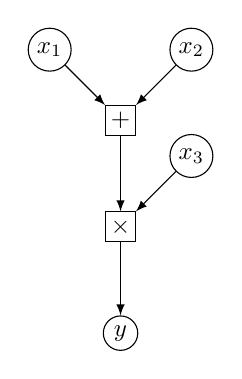
\begin{tikzpicture}[
      scale=0.9, transform shape, >=latex,
      var/.style={draw,circle,minimum size=12pt,inner sep=2pt},
      op/.style={draw,rectangle,minimum width=12pt,minimum height=12pt,inner sep=2pt}
  ]
      % 좌표 배치
      \node[var] (x1) at (0,0) {$x_1$};
      \node[var] (x2) at (2,0) {$x_2$};
      \node[op]  (add) at (1,-1.0) {+};

      \node[var] (x3) at (2,-1.5) {$x_3$};
      \node[op]  (mul) at (1,-2.5) {$\times$};
      \node[var] (y)   at (1,-4.0) {$y$};

      % 연결
      \draw[->] (x1) -- (add);
      \draw[->] (x2) -- (add);
      \draw[->] (add) -- (mul);
      \draw[->] (x3) -- (mul);
      \draw[->] (mul) -- (y);
  \end{tikzpicture}
  \end{column}

\end{columns}
\end{frame}

% Slide 24: requires_grad and Leaf Tensors
\begin{frame}[fragile]{requires\_grad and Leaf Tensors}
\begin{lstlisting}
# Leaf tensors (user-created with requires_grad=True)
x = torch.randn(3, requires_grad=True)
w = torch.randn(3, 4, requires_grad=True)

# Non-leaf tensors (results of operations)
y = x @ w.T               # y.requires_grad = True (inherited)
z = y.sum()              # z.requires_grad = True

# Check tensor properties
print(x.is_leaf)         # True
print(y.is_leaf)         # False
print(x.grad_fn)         # None (leaf tensor)
print(y.grad_fn)         # <MmBackward>

# Gradients accumulate only in leaf tensors
z.backward()
print(x.grad)            # Has gradient
print(y.grad)            # None (non-leaf)
\end{lstlisting}
\end{frame}

% Slide 25: Backward Pass
\begin{frame}[fragile]{The Backward Pass}
\begin{lstlisting}
# Simple example
x = torch.tensor([2.0], requires_grad=True)
y = x ** 2                # y = x^2
z = 2 * y                 # z = 2x^2

# Compute gradients
z.backward()              # dz/dx = 4x = 8

print(x.grad)             # tensor([8.])

# Gradient accumulation (be careful!)
x.grad.zero_()           # Reset gradient
y2 = x ** 3
y2.backward()
print(x.grad)            # tensor([12.]) = 3x^2

# Multiple backwards require retain_graph
loss1 = (x ** 2).sum()
loss2 = (x ** 3).sum()
loss1.backward(retain_graph=True)
loss2.backward()         # Works because of retain_graph
\end{lstlisting}
\end{frame}

% Slide 26: Chain Rule in Action
\begin{frame}[fragile]{Chain Rule in Action}
\begin{lstlisting}
# Multi-layer computation
x = torch.randn(2, 3, requires_grad=True)
W1 = torch.randn(4, 3, requires_grad=True)
W2 = torch.randn(5, 4, requires_grad=True)

# Forward pass
h = torch.relu(x @ W1.T)     # [2, 4]
y = h @ W2.T                  # [2, 5]
loss = y.mean()               # scalar

# Backward pass applies chain rule
loss.backward()

# Gradients computed via chain rule:
# dL/dW2 = dL/dy * dy/dW2
# dL/dW1 = dL/dy * dy/dh * dh/dW1
# dL/dx = dL/dy * dy/dh * dh/dx

print(W2.grad.shape)          # [5, 4]
print(W1.grad.shape)          # [4, 3]
print(x.grad.shape)           # [2, 3]
\end{lstlisting}
\end{frame}

% Slide 27: Gradient Flow Control
\begin{frame}[fragile]{Controlling Gradient Flow}
\begin{lstlisting}
# Stop gradients with detach()
x = torch.randn(3, requires_grad=True)
y = x ** 2
z = y.detach()           # Stop gradient here
w = z * 2

w.sum().backward()       # No gradient flows to x
print(x.grad)            # None

# Stop gradients with torch.no_grad()
x = torch.randn(3, requires_grad=True)
with torch.no_grad():
    y = x ** 2           # No graph built
print(y.requires_grad)   # False

# Gradient clipping (prevent exploding gradients)
torch.nn.utils.clip_grad_norm_(parameters, max_norm=1.0)
torch.nn.utils.clip_grad_value_(parameters, clip_value=1.0)
\end{lstlisting}
\end{frame}

% Slide 28: Common Autograd Patterns
\begin{frame}[fragile]{Common Autograd Patterns}
\begin{lstlisting}
# Pattern 1: Training loop
for epoch in range(num_epochs):
    optimizer.zero_grad()        # Clear gradients
    output = model(input)        # Forward pass
    loss = criterion(output, target)
    loss.backward()              # Compute gradients
    optimizer.step()             # Update weights

# Pattern 2: Gradient accumulation
accumulation_steps = 4
for i, (input, target) in enumerate(dataloader):
    output = model(input)
    loss = criterion(output, target) / accumulation_steps
    loss.backward()
    
    if (i + 1) % accumulation_steps == 0:
        optimizer.step()
        optimizer.zero_grad()
\end{lstlisting}
\end{frame}

% Slide 29: Higher-Order Gradients
\begin{frame}[fragile]{Higher-Order Gradients}
\begin{lstlisting}
# Second-order gradients (Hessian)
x = torch.randn(3, requires_grad=True)
y = (x ** 3).sum()

# First derivative
grad = torch.autograd.grad(y, x, create_graph=True)[0]
print(grad)              # 3x^2

# Second derivative
grad2 = torch.autograd.grad(grad.sum(), x)[0]
print(grad2)             # 6x

# Using backward twice
x = torch.randn(3, requires_grad=True)
y = (x ** 4).sum()
y.backward(create_graph=True)
first_grad = x.grad.clone()
x.grad.sum().backward()
second_grad = x.grad - first_grad
\end{lstlisting}
\end{frame}

% Slide 30: Custom Autograd Functions
\begin{frame}[fragile]{Custom Autograd Functions}
\begin{lstlisting}
class CustomReLU(torch.autograd.Function):
    @staticmethod
    def forward(ctx, input):
        ctx.save_for_backward(input)
        return input.clamp(min=0)
    
    @staticmethod
    def backward(ctx, grad_output):
        input, = ctx.saved_tensors
        grad_input = grad_output.clone()
        grad_input[input < 0] = 0
        return grad_input

# Use custom function
custom_relu = CustomReLU.apply
x = torch.randn(5, requires_grad=True)
y = custom_relu(x)
y.sum().backward()
print(x.grad)  # Gradient only where x > 0
\end{lstlisting}
\end{frame}

% Slide 31: Gradient Checking
\begin{frame}[fragile]{Gradient Checking}
\begin{lstlisting}
def gradient_check(f, x, eps=1e-6):
    """Check gradients using finite differences"""
    # Analytic gradient via autograd
    x.requires_grad = True
    y = f(x)
    y.backward()
    analytic_grad = x.grad.clone()
    
    # Numerical gradient
    x.requires_grad = False
    numerical_grad = torch.zeros_like(x)
    
    for i in range(x.numel()):
        x_pos = x.clone()
        x_pos.view(-1)[i] += eps
        x_neg = x.clone()
        x_neg.view(-1)[i] -= eps
        numerical_grad.view(-1)[i] = (f(x_pos) - f(x_neg)) / (2 * eps)
    
    # Compare
    error = (analytic_grad - numerical_grad).abs().max()
    return error < 1e-4
\end{lstlisting}
\end{frame}

% Slide 32: Memory Management
\begin{frame}[fragile]{Memory Management with Autograd}
\begin{lstlisting}
# Memory-efficient gradient computation
# Problem: Large intermediate tensors
x = torch.randn(1000, 1000, requires_grad=True)
y = x @ x @ x @ x  # Many intermediates stored

# Solution 1: Gradient checkpointing
from torch.utils.checkpoint import checkpoint

def expensive_function(x):
    return x @ x @ x @ x

# Recompute intermediates during backward
y = checkpoint(expensive_function, x)

# Solution 2: In-place operations (use carefully!)
x = torch.randn(1000, 1000)
x.requires_grad = True
# x.add_(1)  # ERROR: Can't use in-place on leaf
y = x.clone()
y.add_(1)    # OK: In-place on non-leaf
\end{lstlisting}
\end{frame}

% Slide 33: Debugging Autograd
\begin{frame}[fragile]{Debugging Autograd Issues}
\begin{lstlisting}
# Common issues and solutions

# 1. None gradients
x = torch.randn(3)  # No requires_grad!
y = x ** 2
y.backward()  # ERROR: requires_grad needed

# 2. Gradient not flowing
x = torch.randn(3, requires_grad=True)
y = x.detach() ** 2  # Detach breaks flow
y.backward()  # ERROR: grad_fn is None

# 3. In-place operation error
x = torch.randn(3, requires_grad=True)
y = x ** 2
x[0] = 0  # ERROR: In-place on needed tensor

# 4. Double backward without retain_graph
loss.backward()
loss.backward()  # ERROR: Graph already freed
\end{lstlisting}
\end{frame}

% Slide 34: Autograd Profiler
\begin{frame}[fragile]{Profiling Autograd Operations}
\begin{lstlisting}
import torch.autograd.profiler as profiler

# Profile forward and backward passes
with profiler.profile(use_cuda=torch.cuda.is_available()) as prof:
    x = torch.randn(100, 100, requires_grad=True)
    y = x @ x
    z = y.sum()
    z.backward()

# Print profiling results
print(prof.key_averages().table(sort_by="cpu_time_total"))

# Export to Chrome tracing
prof.export_chrome_trace("trace.json")

# Record specific operations
with profiler.record_function("my_operation"):
    result = expensive_computation()
\end{lstlisting}
\end{frame}

% Slide 35: Section Summary
\begin{frame}{Automatic Differentiation Summary}
\begin{block}{Key Concepts}
\begin{itemize}
    \item Dynamic computational graphs
    \item Forward pass builds graph, backward computes gradients
    \item requires\_grad enables gradient tracking
    \item Chain rule automatically applied
    \item Gradient accumulation and flow control
\end{itemize}
\end{block}

\begin{alertblock}{Best Practices}
\begin{itemize}
    \item Always zero gradients before backward
    \item Use torch.no\_grad() for inference
    \item Detach tensors to stop gradient flow
    \item Check gradients with finite differences
    \item Profile to find bottlenecks
\end{itemize}
\end{alertblock}
\end{frame}

% ============================================
% SECTION 3: Neural Network Modules (Slides 36-50)
% ============================================
\section{Neural Network Modules}

% Slide 36: Section introduction
\begin{frame}{Neural Network Modules}
\begin{center}
\Large{Building Blocks of Deep Learning}
\end{center}

\begin{block}{Topics}
\begin{itemize}
    \item nn.Module architecture
    \item Common layers and activation functions
    \item Loss functions and optimizers
    \item Training patterns and best practices
\end{itemize}
\end{block}
\end{frame}

% Slide 37: nn.Module Basics
\begin{frame}[fragile]{nn.Module Basics}
\begin{lstlisting}
import torch.nn as nn

class SimpleNet(nn.Module):
    def __init__(self, input_dim, hidden_dim, output_dim):
        super(SimpleNet, self).__init__()
        self.fc1 = nn.Linear(input_dim, hidden_dim)
        self.relu = nn.ReLU()
        self.fc2 = nn.Linear(hidden_dim, output_dim)
    
    def forward(self, x):
        x = self.fc1(x)
        x = self.relu(x)
        x = self.fc2(x)
        return x

# Create and use model
model = SimpleNet(10, 20, 5)
x = torch.randn(32, 10)  # [batch, input_dim]
output = model(x)         # [batch, output_dim]
\end{lstlisting}
\end{frame}

% Slide 38: Common Layers
\begin{frame}[fragile]{Common Layer Types}
\begin{lstlisting}
# Linear layers
linear = nn.Linear(10, 20, bias=True)

# Convolutional layers
conv1d = nn.Conv1d(in_channels=3, out_channels=16, kernel_size=5)
conv2d = nn.Conv2d(3, 32, kernel_size=3, padding=1)

# Recurrent layers
lstm = nn.LSTM(input_size=10, hidden_size=20, num_layers=2)
gru = nn.GRU(10, 20, batch_first=True)

# Normalization layers
batch_norm = nn.BatchNorm1d(20)
layer_norm = nn.LayerNorm([20])

# Dropout for regularization
dropout = nn.Dropout(p=0.5)
\end{lstlisting}
\end{frame}

% Slide 39: Activation Functions
\begin{frame}[fragile]{Activation Functions}
\begin{lstlisting}
# Common activations
relu = nn.ReLU()
sigmoid = nn.Sigmoid()
tanh = nn.Tanh()
softmax = nn.Softmax(dim=1)

# Advanced activations
leaky_relu = nn.LeakyReLU(negative_slope=0.01)
elu = nn.ELU(alpha=1.0)
gelu = nn.GELU()
swish = nn.SiLU()  # Also known as Swish

# In functional form
import torch.nn.functional as F
x = torch.randn(10, 20)
y = F.relu(x)
z = F.softmax(x, dim=1)
\end{lstlisting}
\end{frame}

% Slide 40: Loss Functions
\begin{frame}[fragile]{Loss Functions}
\begin{lstlisting}
# Regression losses
mse_loss = nn.MSELoss()
l1_loss = nn.L1Loss()
smooth_l1 = nn.SmoothL1Loss()  # Huber loss

# Classification losses
cross_entropy = nn.CrossEntropyLoss()
nll_loss = nn.NLLLoss()
bce_loss = nn.BCELoss()
bce_with_logits = nn.BCEWithLogitsLoss()

# Example usage
predictions = model(inputs)      # [batch, classes]
targets = torch.randint(0, 10, (batch_size,))
loss = cross_entropy(predictions, targets)

# Custom weights for imbalanced classes
weights = torch.tensor([1.0, 2.0, 1.5])
weighted_ce = nn.CrossEntropyLoss(weight=weights)
\end{lstlisting}
\end{frame}

% Slide 41: Optimizers
\begin{frame}[fragile]{Optimizers}
\begin{lstlisting}
# Common optimizers
sgd = torch.optim.SGD(model.parameters(), lr=0.01, 
                       momentum=0.9, weight_decay=1e-4)
adam = torch.optim.Adam(model.parameters(), lr=1e-3,
                        betas=(0.9, 0.999), eps=1e-8)
rmsprop = torch.optim.RMSprop(model.parameters(), lr=0.01)
adamw = torch.optim.AdamW(model.parameters(), lr=1e-3,
                          weight_decay=0.01)

# Learning rate scheduling
scheduler = torch.optim.lr_scheduler.StepLR(optimizer, 
                                           step_size=30, gamma=0.1)
cosine_scheduler = torch.optim.lr_scheduler.CosineAnnealingLR(
                                optimizer, T_max=100)

# Update learning rate
for epoch in range(num_epochs):
    train_epoch()
    scheduler.step()
\end{lstlisting}
\end{frame}

% Slide 42: Parameter Management
\begin{frame}[fragile]{Parameter Management}
\begin{lstlisting}
# Access parameters
for name, param in model.named_parameters():
    print(name, param.shape)

# Freeze parameters
for param in model.fc1.parameters():
    param.requires_grad = False

# Count parameters
total_params = sum(p.numel() for p in model.parameters())
trainable_params = sum(p.numel() for p in model.parameters() 
                      if p.requires_grad)

# Parameter groups with different learning rates
optimizer = torch.optim.Adam([
    {'params': model.fc1.parameters(), 'lr': 1e-4},
    {'params': model.fc2.parameters(), 'lr': 1e-3}
])
\end{lstlisting}
\end{frame}

% Slide 43: Weight Initialization
\begin{frame}[fragile]{Weight Initialization}
\begin{lstlisting}
# Xavier/Glorot initialization
def init_weights_xavier(m):
    if isinstance(m, nn.Linear):
        nn.init.xavier_uniform_(m.weight)
        if m.bias is not None:
            nn.init.zeros_(m.bias)

# He/Kaiming initialization (better for ReLU)
def init_weights_he(m):
    if isinstance(m, nn.Linear):
        nn.init.kaiming_normal_(m.weight, mode='fan_out',
                               nonlinearity='relu')
        if m.bias is not None:
            nn.init.zeros_(m.bias)

# Apply to model
model.apply(init_weights_he)

# Custom initialization
model.fc1.weight.data.normal_(0, 0.01)
model.fc1.bias.data.fill_(0)
\end{lstlisting}
\end{frame}

% Slide 44: Regularization Techniques
\begin{frame}[fragile]{Regularization Techniques}
\begin{lstlisting}
class RegularizedNet(nn.Module):
    def __init__(self, input_dim, hidden_dim, output_dim,
                 dropout_rate=0.5):
        super().__init__()
        self.fc1 = nn.Linear(input_dim, hidden_dim)
        self.dropout1 = nn.Dropout(dropout_rate)
        self.bn1 = nn.BatchNorm1d(hidden_dim)
        self.fc2 = nn.Linear(hidden_dim, output_dim)
        
    def forward(self, x):
        x = self.fc1(x)
        x = self.bn1(x)
        x = F.relu(x)
        x = self.dropout1(x)
        x = self.fc2(x)
        return x

# L2 regularization via weight_decay
optimizer = torch.optim.Adam(model.parameters(),
                            weight_decay=1e-4)
\end{lstlisting}
\end{frame}

% Slide 45: Training Pattern
\begin{frame}[fragile]{Complete Training Pattern}
\begin{lstlisting}
def train_epoch(model, dataloader, optimizer, criterion):
    model.train()  # Set to training mode
    total_loss = 0
    
    for batch_idx, (data, target) in enumerate(dataloader):
        data, target = data.to(device), target.to(device)
        
        # Forward pass
        optimizer.zero_grad()
        output = model(data)
        loss = criterion(output, target)
        
        # Backward pass
        loss.backward()
        torch.nn.utils.clip_grad_norm_(model.parameters(), 1.0)
        optimizer.step()
        
        total_loss += loss.item()
    
    return total_loss / len(dataloader)
\end{lstlisting}
\end{frame}

% Slide 46: Evaluation Pattern
\begin{frame}[fragile]{Evaluation Pattern}
\begin{lstlisting}
def evaluate(model, dataloader, criterion):
    model.eval()  # Set to evaluation mode
    total_loss = 0
    correct = 0
    
    with torch.no_grad():  # Disable gradient computation
        for data, target in dataloader:
            data, target = data.to(device), target.to(device)
            
            output = model(data)
            loss = criterion(output, target)
            total_loss += loss.item()
            
            # Calculate accuracy
            pred = output.argmax(dim=1)
            correct += pred.eq(target).sum().item()
    
    accuracy = 100. * correct / len(dataloader.dataset)
    avg_loss = total_loss / len(dataloader)
    return avg_loss, accuracy
\end{lstlisting}
\end{frame}

% Slide 47: Model Persistence
\begin{frame}[fragile]{Saving and Loading Models}
\begin{lstlisting}
# Save model state dict (recommended)
torch.save(model.state_dict(), 'model.pth')

# Load model state dict
model = SimpleNet(input_dim, hidden_dim, output_dim)
model.load_state_dict(torch.load('model.pth'))

# Save complete checkpoint
checkpoint = {
    'epoch': epoch,
    'model_state_dict': model.state_dict(),
    'optimizer_state_dict': optimizer.state_dict(),
    'loss': loss,
    'best_accuracy': best_accuracy
}
torch.save(checkpoint, 'checkpoint.pth')

# Load checkpoint
checkpoint = torch.load('checkpoint.pth')
model.load_state_dict(checkpoint['model_state_dict'])
optimizer.load_state_dict(checkpoint['optimizer_state_dict'])
\end{lstlisting}
\end{frame}

% Slide 48: Mixed Precision Training
\begin{frame}[fragile]{Mixed Precision Training}
\begin{lstlisting}
from torch.cuda.amp import autocast, GradScaler

# Initialize scaler for mixed precision
scaler = GradScaler()

for epoch in range(num_epochs):
    for batch_idx, (data, target) in enumerate(dataloader):
        optimizer.zero_grad()
        
        # Mixed precision forward pass
        with autocast():
            output = model(data)
            loss = criterion(output, target)
        
        # Scaled backward pass
        scaler.scale(loss).backward()
        scaler.step(optimizer)
        scaler.update()

# Note: Only beneficial on GPUs with Tensor Cores
# (NVIDIA V100, RTX 20xx, 30xx, 40xx, A100, etc.)
\end{lstlisting}
\end{frame}

% Slide 49: Model Compilation (PyTorch 2.0+)
\begin{frame}[fragile]{Model Compilation with torch.compile}
\begin{lstlisting}
# PyTorch 2.0+ feature for faster execution
import torch

# Compile model for optimization
model = SimpleNet(input_dim, hidden_dim, output_dim)
compiled_model = torch.compile(model)

# Different compilation modes
model_reduce = torch.compile(model, mode="reduce-overhead")
model_max = torch.compile(model, mode="max-autotune")

# Disable for debugging
model_default = torch.compile(model, mode="default",
                             disable=True)

# Backend options
model_inductor = torch.compile(model, backend="inductor")

# Note: First run will be slower (compilation overhead)
# Subsequent runs will be significantly faster
\end{lstlisting}
\end{frame}

% Slide 50: Section Summary
\begin{frame}{Neural Network Modules Summary}
\begin{block}{Key Components}
\begin{itemize}
    \item nn.Module as base class for all models
    \item Layers, activations, loss functions, optimizers
    \item Weight initialization strategies
    \item Regularization: dropout, batch norm, weight decay
    \item Training and evaluation patterns
\end{itemize}
\end{block}

\begin{alertblock}{Best Practices}
\begin{itemize}
    \item Always set model.train() and model.eval()
    \item Use torch.no\_grad() during evaluation
    \item Initialize weights appropriately
    \item Save and load checkpoints regularly
    \item Consider mixed precision for large models
\end{itemize}
\end{alertblock}
\end{frame}

% ============================================
% SECTION 4: Hands-on Experiments (Slides 51-70)
% ============================================
\section{Hands-on Experiments}

% Slide 51: Experiments Overview
\begin{frame}{Hands-on Experiments}
\begin{center}
\Large{9 Progressive Experiments}
\end{center}

\begin{enumerate}
    \item Environment setup and sanity checks (exp01)
    \item Tensors and automatic differentiation (exp02)
    \item Computational graph visualization (exp03)
    \item Building nn.Module networks (exp04)
    \item Loss functions and optimizers (exp05)
    \item Regularization and initialization (exp06)
    \item Complete training pipeline (exp07)
    \item Mixed precision and compilation (exp08)
    \item Integration test (exp09)
\end{enumerate}
\end{frame}

% Slide 52-53: Experiment 1
\begin{frame}{Experiment 1: Setup and Sanity Checks}
\textbf{Goal:} Verify environment and basic operations

\textbf{Tasks:}
\begin{itemize}
    \item Check PyTorch installation and version
    \item Test device availability (CPU/CUDA/MPS)
    \item Verify tensor operations
    \item Test reproducibility with seeds
\end{itemize}

\textbf{Run:} \texttt{python exp01\_setup.py}

\textbf{Expected:} Device detected, operations successful
\end{frame}

\begin{frame}[fragile]{Exp1: Key Code}
\begin{lstlisting}
def main():
    print("="*50)
    print("Experiment 01: Setup and Sanity")
    print("="*50)
    
    # Device selection
    device = torch.device(
        'cuda' if torch.cuda.is_available() 
        else 'mps' if hasattr(torch.backends, 'mps') 
                      and torch.backends.mps.is_available()
        else 'cpu'
    )
    print(f"Using device: {device}")
    
    # Test operations
    x = torch.randn(3, 4).to(device)
    y = x @ x.T
    print(f"Matrix multiply OK, shape: {y.shape}")
\end{lstlisting}
\end{frame}

% Slides 54-55: Experiment 2
\begin{frame}{Experiment 2: Tensors and Autograd}
\textbf{Goal:} Master tensor operations and gradients

\textbf{Tasks:}
\begin{itemize}
    \item Create tensors with gradient tracking
    \item Perform operations and compute gradients
    \item Understand gradient accumulation
    \item Test gradient flow control
\end{itemize}

\textbf{Key Learning:} How autograd tracks operations
\end{frame}

\begin{frame}[fragile]{Exp2: Key Code}
\begin{lstlisting}
# Automatic differentiation example
x = torch.tensor([2.0, 3.0], requires_grad=True)
y = x ** 2
z = y.sum()

z.backward()
print(f"x.grad = {x.grad}")  # [4.0, 6.0]

# Gradient accumulation
x.grad.zero_()
for i in range(3):
    y = (x ** 2).sum()
    y.backward()
print(f"Accumulated grad = {x.grad}")  # [12.0, 18.0]
\end{lstlisting}
\end{frame}

% Slides 56-57: Experiment 3
\begin{frame}{Experiment 3: Computational Graph}
\textbf{Goal:} Visualize and understand computation graphs

\textbf{Tasks:}
\begin{itemize}
    \item Build complex computational graphs
    \item Inspect grad\_fn attributes
    \item Trace backward pass
    \item Understand graph retention
\end{itemize}

\textbf{Critical:} Graphs are dynamic and rebuilt each forward
\end{frame}

% Slides 58-59: Experiment 4
\begin{frame}{Experiment 4: nn.Module Networks}
\textbf{Goal:} Build custom neural networks

\textbf{Components tested:}
\begin{itemize}
    \item Custom nn.Module classes
    \item Parameter management
    \item Forward pass implementation
    \item Model composition
\end{itemize}

\textbf{Expected outcome:} Working multi-layer network
\end{frame}

% Slides 60-61: Experiment 5
\begin{frame}{Experiment 5: Losses and Optimizers}
\textbf{Goal:} Compare different losses and optimizers

\textbf{Components:}
\begin{itemize}
    \item MSE, Cross-entropy, Huber losses
    \item SGD, Adam, AdamW optimizers
    \item Learning rate scheduling
    \item Gradient clipping
\end{itemize}

Compare convergence rates and stability
\end{frame}

% Slides 62-63: Experiment 6
\begin{frame}{Experiment 6: Regularization}
\textbf{Goal:} Apply regularization techniques

\textbf{Features:}
\begin{itemize}
    \item Dropout layers
    \item Batch normalization
    \item Weight decay (L2 regularization)
    \item Different initialization strategies
\end{itemize}

Observe effects on training and validation loss
\end{frame}

% Slides 64-65: Experiment 7
\begin{frame}{Experiment 7: Training Pipeline}
\textbf{Goal:} Complete training and evaluation loop

\textbf{What to implement:}
\begin{itemize}
    \item Data loading with DataLoader
    \item Training loop with metrics
    \item Validation with early stopping
    \item Checkpoint saving
\end{itemize}

Full end-to-end training workflow
\end{frame}

% Slides 66-67: Experiment 8
\begin{frame}{Experiment 8: Advanced Features}
\textbf{Goal:} Use PyTorch 2.0+ features

\textbf{Best practices:}
\begin{itemize}
    \item Mixed precision training (AMP)
    \item Model compilation with torch.compile
    \item Profiling and optimization
    \item Memory-efficient training
\end{itemize}
\end{frame}

% Slides 68-70: Experiment 9 (Integration Test)
\begin{frame}{Experiment 9: Integration Test}
\textbf{Goal:} Validate complete implementation

\textbf{Tests performed:}
\begin{enumerate}
    \item Device management and reproducibility
    \item Tensor operations and autograd
    \item Model construction and initialization
    \item Loss computation and optimization
    \item Training and evaluation loops
    \item Checkpoint save/load functionality
\end{enumerate}

Must pass all tests before proceeding!
\end{frame}

\begin{frame}[fragile]{Exp9: Expected Output}
\begin{lstlisting}
# Run integrated test
python exp09_integrated_test.py

# Expected output:
# =====================================
# Test 1: Device Setup         [PASS]
# Test 2: Autograd            [PASS]
# Test 3: nn.Module           [PASS]
# Test 4: Optimization        [PASS]
# Test 5: Training Loop       [PASS]
# Test 6: Checkpointing       [PASS]
# =====================================
# All tests passed!
\end{lstlisting}
\end{frame}

% ============================================
% WRAP-UP (Slides 71-75)
% ============================================
\section{Wrap-up}

% Slide 71: Key Takeaways
\begin{frame}{Key Takeaways}
\begin{enumerate}
    \item \textbf{Tensors:} Foundation of all computations in PyTorch
    \item \textbf{Autograd:} Automatic differentiation via dynamic graphs
    \item \textbf{Device Management:} Always check CUDA > MPS > CPU
    \item \textbf{nn.Module:} Building block for all neural networks
    \item \textbf{Training Pattern:} zero\_grad, forward, backward, step
    \item \textbf{Best Practices:} Reproducibility, checkpointing, profiling
\end{enumerate}
\end{frame}

\end{document}